%
% section 4.1.1
%
\subsection{Πρωτόκολλο TCP -- Δομή Πακέτου}

\begin{inthebox}
\textbf{Προσοχή:} Η αντίστοιχη ενότητα στο βιβλίο περιέχει διάφορα λάθη και ανακρίβειες, έχοντας ανακατέψει τις λειτουργίες των επιπέδων Μεταφοράς και Διαδικτύου. Σε αυτή την παράγραφο γράφουμε την πραγματικότητα, χρησιμοποιώντας το παράδειγμα του βιβλίου.\\
\end{inthebox}


\emph{Παράδειγμα Σχολικού Βιβλίου:} Έστω ότι θέλουμε να αποστείλουμε ένα μήνυμα μέσω ηλεκτρονικού ταχυδρομείου. Ο χρήστης θα γράψει το μήνυμα του στην αντίστοιχη εφαρμογή και θα συμπληρώσει την διεύθυνση ηλεκτρονικού ταχυδρομείου του παραλήπτη. Η διεύθυνση αυτή (μαζί με την αντίστοιχη του αποστολέα) αποτελούν μέρος της επικεφαλίδας που προστίθεται στο μήνυμα που δημιουργείται από το επίπεδο εφαρμογής.

Θυμηθείτε ότι το επίπεδο εφαρμογής, λειτουργεί με εντολές που είναι γενικά κατανοητές από τον άνθρωπο: τα προγράμματα σε αυτό το επίπεδο συνεννοούνται κατά βάση με εντολές στα αγγλικά που μπορούμε πολλές φορές να στείλουμε και χειροκίνητα. Για παράδειγμα μια συνομιλία με ένα διακομιστή ηλεκτρονικού ταχυδρομείου ξεκινά με το χαιρετισμό ``helo'' (ναι, είναι με ένα ``l'') ή ``ehlo''. Όλες αυτές οι εντολές και τα δεδομένα (κείμενο) του χρήστη πρέπει ωστόσο να μεταφερθούν μέσα από το επίπεδο μεταφοράς.

Το επίπεδο εφαρμογής δεν ενδιαφέρεται -- και δεν γνωρίζει -- τους περιορισμούς του φυσικού μέσου. Όσο αφορά ένα πρόγραμμα ταχυδρομείου, ο χρήστης μπορεί να γράψει και να στείλει όσο μεγάλο (ή μικρό) μήνυμα θέλει. Το πρόγραμμα επικοινωνεί απευθείας με το αντίστοιχο στην άλλη μεριά: οι λεπτομέρειες της πραγματικής επικοινωνίας κρύβονται στα παρακάτω επίπεδα.

Ας υποθέσουμε λοιπόν ότι ο χρήστης έγραψε ένα μήνυμα μεγέθους 6000 octets (ή bytes, αν το προτιμάτε). Το επίπεδο μεταφοράς θα πρέπει να τα μεταφέρει μέσω του TCP, αφού πρώτα γίνει μια αρχική σύνδεση και συννενόηση με τον παραλήπτη (το TCP είναι πρωτόκολλο με σύνδεση). Με ποιο τρόπο και για ποιο λόγο θα αποφασίσει το TCP να δημιουργήσει τη δική του μονάδα δεδομένων (τα τμήματα, ή segments) με κάποιο συγκεκριμένο μέγεθος; Θα μπορούσε να στείλει όλο το μήνυμα σε ένα τμήμα;

Σύμφωνα με αυτά που ξέρουμε η απάντηση είναι ναι: Το TCP μπορεί να δημιουργήσει ένα τμήμα των 6000 bytes: τα τμήματα του TCP ενθυλακώνονται πάντα σε αυτοδύναμα πακέτα IP, και αυτά με τη σειρά τους ενθυλακώνονται στην αντίστοιχη μονάδα δεδομένων του κατώτερου επίπεδου (π.χ. σε πλαίσια Ethernet). Στο επίπεδο Διαδικτύου, τα πακέτα IP μπορούν να υποστούν κατάτμηση (fragmentation) αν το μέγεθος τους είναι τέτοιο που δεν μπορούν να ενθυλακωθούν σε πλαίσια. Θα μπορούσε λοιπόν το TCP να αφήσει αυτή τη λειτουργία στο IP. Υπάρχει λόγος να μην το κάνει;

Ναι. Όταν τα αυτοδύναμα πακέτα IP διασπώνται σε fragments, η απόδοση μειώνεται. Το κάθε fragment έχει δική του επικεφαλίδα και άρα μεταφέρει λιγότερα χρήσιμα δεδομένα από ότι ένα μη-διασπασμένο αυτοδύναμο πακέτο. Επίσης αν ένα fragment χαθεί ή καταστραφεί, είναι πλέον αδύνατο να συναρμολογηθεί το αντίστοιχο αυτοδύναμο πακέτο. Όμως αυτό το πακέτο έχει μέσα του πολλά δεδομένα (ένα ολόκληρο ``μεγάλου μεγέθους'' τμήμα): το επίπεδο μεταφοράς θα χρειαστεί να ξαναστείλει όλο το τμήμα.

Για να βελτιστοποιήσουμε την απόδοση, στην έναρξη της επικοινωνίας και οι δυο μεριές δηλώνουν το μέγιστο μέγεθος τμήματος που μπορούν να χρησιμοποιήσουν. Αυτό είναι γενικά γνωστό ως Maximum Segment Size (MSS). Δεν γίνεται κάποια διαπραγμάτευση μεταξύ των δύο άκρων: είναι απλά μια δήλωση. Σε γενικές γραμμές, επιλέγεται μια τιμή τέτοια ώστε να μη χρειαστεί να γίνει IP fragmentation: μια τέτοια τιμή προφανώς είναι κοντά στη μέγιστη μονάδα μεταφοράς του φυσικού μέσου (MTU), αφού ληφθούν υπόψη και οι επικεφαλίδες που θα προστεθούν σε κάθε επίπεδο. Σημειώστε ότι δεν θα χρησιμοποιηθεί αναγκαστικά η τιμή MSS για όλα τα τμήματα: απλά είναι η μέγιστη δυνατή. Η πραγματική μπορεί να είναι μικρότερη και ρυθμίζεται από παράγοντες όπως ο έλεγχος ροής (το πεδίο ``παράθυρο'').

Στο παράδειγμα μας, έστω ότι τελικά ανακαλύψαμε ότι μια κατάλληλη τιμή είναι τα 600 bytes. Τα αρχικά δεδομένα (6000 bytes) από το επίπεδο εφαρμογής θα γίνουν 10 τμήματα των 600 bytes στο επίπεδο μεταφοράς. Σε καθένα από αυτά τα 10 τμήματα θα προστεθεί (κατ'ελάχιστον) μια επικεφαλίδα 20 bytes για το TCP και μια ακόμα 20 bytes στο επίπεδο IP. Προφανώς το επίπεδο πρόσβασης δικτύου θα πρέπει να μπορεί να δημιουργήσει πλαίσια με μήκος δεδομένων τουλάχιστον 640 bytes.

\begin{figure}[!ht]
 \centering
 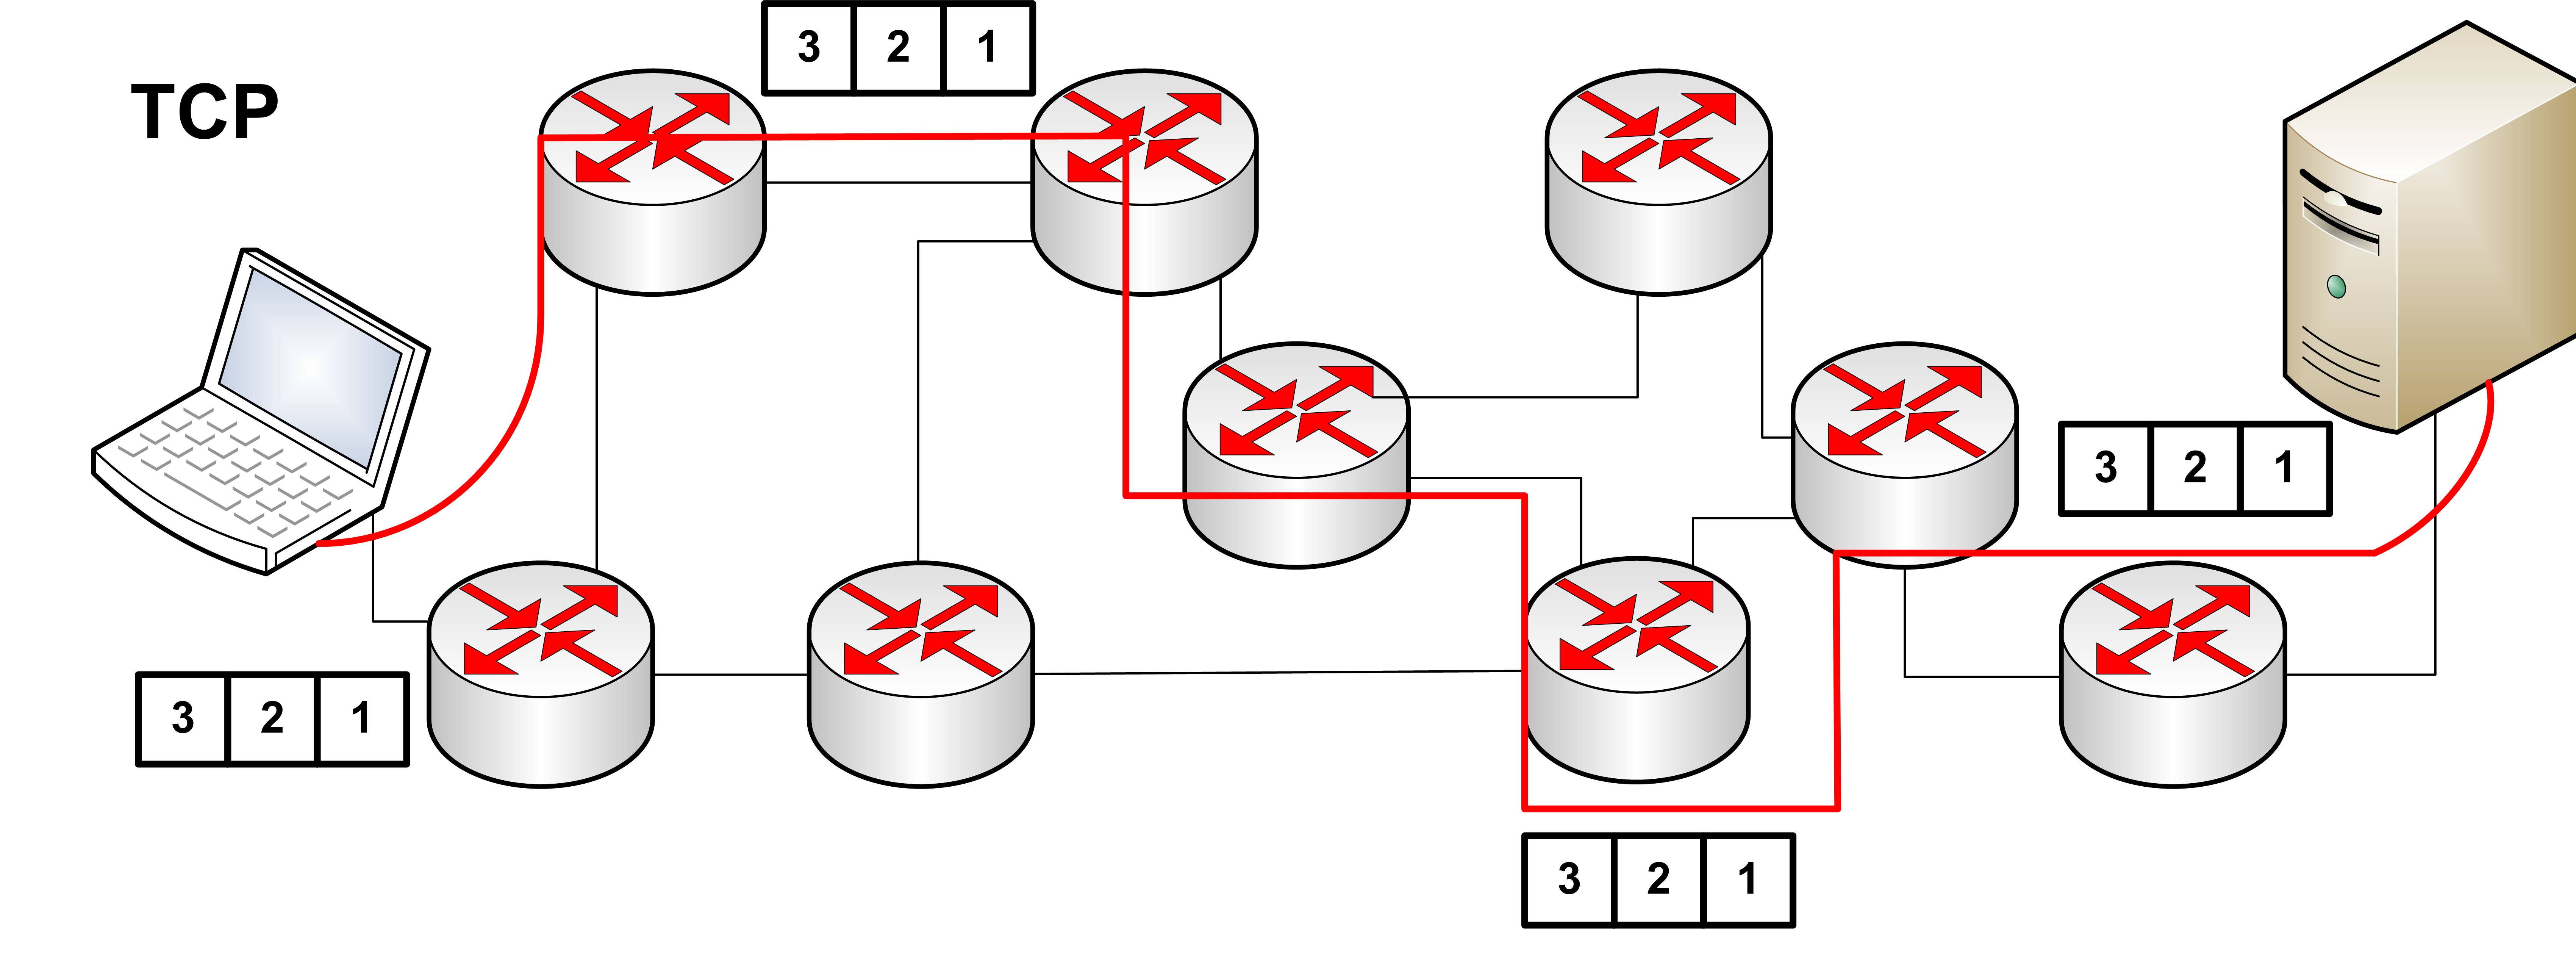
\includegraphics[width=0.85\textwidth]{images/chapter4/4-1-w}
 \caption {\textsl{Επικοινωνία TCP - ΛΑΘΟΣ}}
 \label{4-1-w}
\end{figure}

\begin{figure}[!ht]
 \centering
 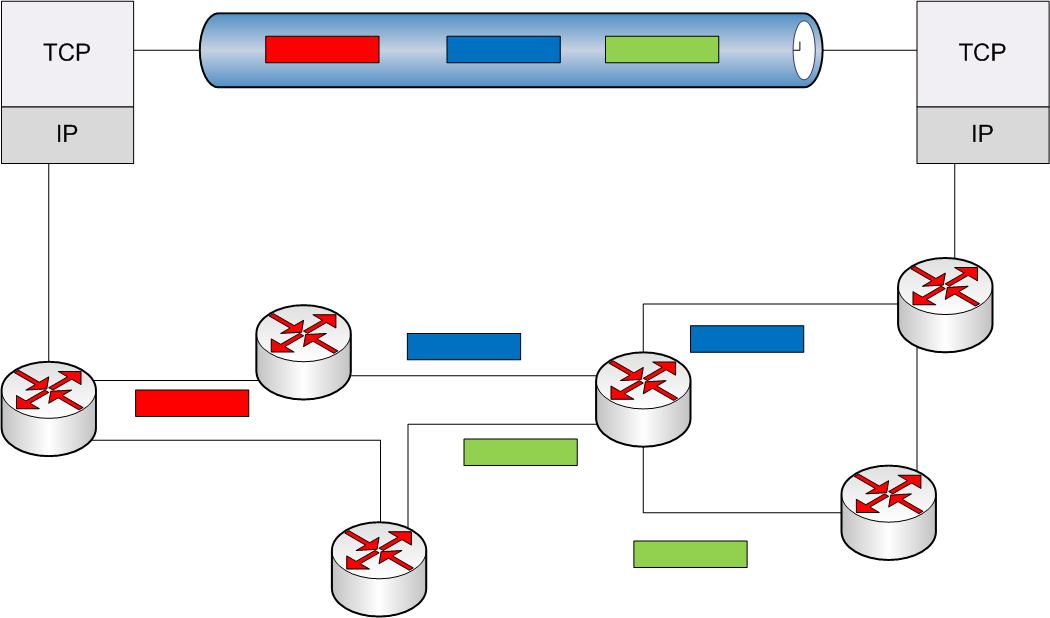
\includegraphics[width=0.85\textwidth]{images/chapter4/4-1-r}
 \caption {\textsl{Επικοινωνία TCP - ΣΩΣΤΗ}}
 \label{4-1-r}
\end{figure}

Η εικόνα \ref{4-1-w} στο βιβλίο σας είναι επίσης λάθος: ο συγγραφέας προσπαθεί να δείξει ότι υπάρχει ένα νοητό κύκλωμα στο TCP αλλά φτιάχνει μια συγκεκριμένη διαδρομή μέσα από δρομολογητές: οι δρομολογητές όμως δεν ασχολούνται με το επίπεδο μεταφοράς αλλά με το επίπεδο διαδικτύου. Όπως γνωρίζουμε το κάθε αυτοδύναμο IP πακέτο αντιμετωπίζεται χωριστά από τους δρομολογητές και πακέτα της ίδιας μετάδοσης μπορεί τελικά να ακολουθήσουν διαφορετικές διαδρομές μέσα από το επικοινωνιακό υποδίκτυο. Η γραμμή που ενώνει εδώ τους κόμβους μέσα από μια συγκεκριμένη διαδρομή είναι άκυρη. Για ένα σωστό σχήμα δείτε την εικόνα \ref{4-1-r} όπου φαίνεται καθαρά ότι όσο αφορά το TCP η επικοινωνία είναι μια ευθεία γραμμή (end to end) αλλά στην πραγματικότητα τα αυτοδύναμα πακέτα μπορεί να κινούνται από διαφορετικές διαδρομές.